\section{Problem Overview}

This project addresses a multi-class news article classification task, where
each document is assigned to one of seven topical categories. The dataset
consists of real-world online news articles in raw HTML format, characterized
by heterogeneous sources, noisy markup, incomplete metadata, and strong
editorial regularities. Performance is evaluated using macro-averaged F1 score
to ensure balanced behavior across classes.

A preliminary exploratory analysis is conducted to identify informative,
redundant, and structurally biased signals, guiding preprocessing and modeling
choices.

\paragraph{Temporal Metadata and Redundancy}
The \textit{timestamp} attribute contains a high proportion of missing values
(\textbf{34.7\%}) and exhibits coarse temporal granularity, with no clear
relationship between fine-grained temporal components and the target labels.
An auxiliary experiment shows that publication year can be predicted directly
from raw article text with approximately \textbf{64.0\%} accuracy, indicating
that temporal information is implicitly encoded in lexical and editorial
patterns. Consequently, explicit timestamp information is treated as redundant
and excluded.

\begin{center}
	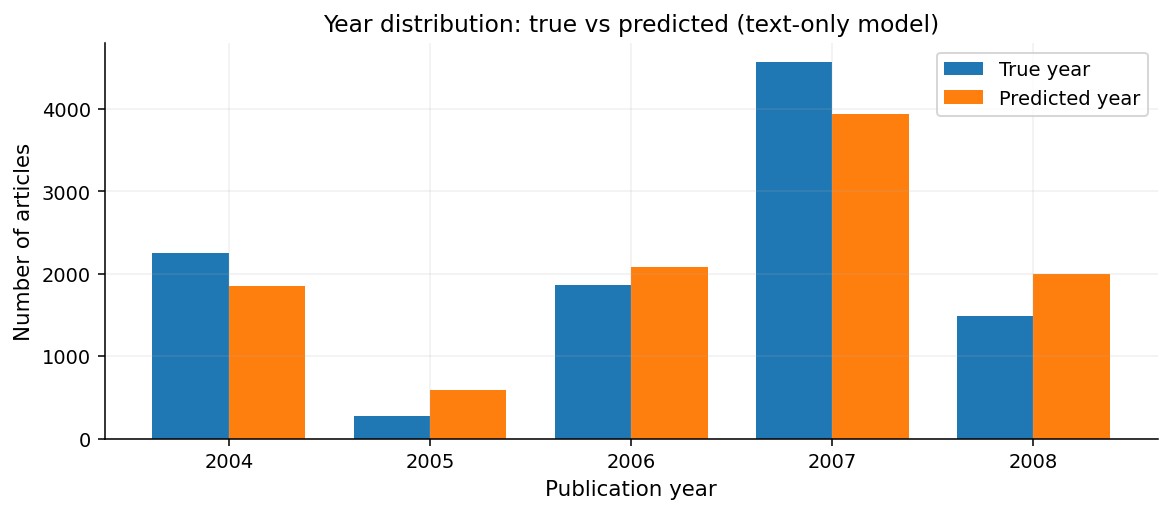
\includegraphics[width=\linewidth]{FIGURES/figure1_year_prediciton.png}
	\captionof{figure}{Distribution of publication years in the development set
	and corresponding predictions obtained from a text-only classifier,
	confirming that temporal information is implicitly encoded in the text.}
	\label{fig:year_prediction}
\end{center}

\paragraph{Non-informative Metadata}
The \textit{page\_rank} feature follows an approximately uniform distribution
and shows no meaningful correlation with the target labels. Its inclusion does
not provide measurable performance gains and is therefore discarded.

\paragraph{Structural Ambiguity}
The dataset contains duplicated or republished articles with identical content
assigned to different labels (\textbf{6.87\%} of the development set). This
introduces intrinsic ambiguity, defining an upper bound on achievable
performance and motivating the use of macro-averaged F1 score.

\paragraph{Editorial Bias and Source Informativeness}
A strong dependency exists between article source and target labels, reflecting
editorial specialization across publishers. One-hot encoding of source
information yields a strong linear baseline, revealing near-deterministic
editorial cues and motivating modeling strategies that separate structurally
deterministic from semantically ambiguous documents.

\textbf{[FIGURE 2 HERE: Source $\times$ Label heatmap]}

\paragraph{Implications}
Overall, the dataset combines noisy HTML-heavy text, redundant metadata, and
strong editorial regularities. These properties motivate a progressive modeling
approach that exploits high-confidence structural signals while reserving more
expressive models for genuinely ambiguous samples.

